\let\negmedspace\undefined
\let\negthickspace\undefined

\documentclass[journal]{IEEEtran}
\usepackage[a5paper, margin=10mm, onecolumn]{geometry}
\usepackage{tfrupee}

\setlength{\headheight}{1cm}
\setlength{\headsep}{0mm}

\usepackage{gvv-book}
\usepackage{gvv}
\usepackage{cite}
\usepackage{amsmath,amssymb,amsfonts,amsthm}
\usepackage{algorithmic}
\usepackage{graphicx}
\usepackage{textcomp}
\usepackage{xcolor}
\usepackage{txfonts}
\usepackage{listings}
\usepackage{enumitem}
\usepackage{mathtools}
\usepackage{gensymb}
\usepackage{comment}
\usepackage[breaklinks=true]{hyperref}
\usepackage{tkz-euclide} 
\usepackage{listings}
\def\inputGnumericTable{}                                 
\usepackage[latin1]{inputenc}                                
\usepackage{color}                                            
\usepackage{array}                                            
\usepackage{longtable}                                       
\usepackage{calc}                                             
\usepackage{multirow}                                         
\usepackage{hhline}                                           
\usepackage{ifthen}                                           
\usepackage{lscape}
\begin{document}

\bibliographystyle{IEEEtran}
\vspace{3cm}

\title{9.4.22}
\author{EE25BTECH11010 - Arsh Dhoke}
{\let\newpage\relax\maketitle}

\renewcommand{\thefigure}{\theenumi}
\renewcommand{\thetable}{\theenumi}
\setlength{\intextsep}{10pt}
\numberwithin{equation}{enumi}
\numberwithin{figure}{enumi}
\renewcommand{\thetable}{\theenumi}

\parindent 0px
\textbf{Question}:\\
Find the value of $k$ such that the quadratic equation
kx(x-2) + 6 = 0 has equal roots. Verify your solution using graph.

\solution \\


\begin{align}
kx^2 - 2kx + 6 = 0
\end{align}

This can be represented as a conic:
\begin{align}
\vec{x}^{T}\vec{V}\vec{x} + 2\vec{u}^{T}\vec{x} + f = 0
\end{align}
where
\begin{align}
\vec{V} = \myvec{k & 0 \\ 0 & 0}, \quad
\vec{u} = \myvec{-k \\ 0}, \quad
f = 6
\end{align}

For the roots of the quadratic to be equal, the line $y=0$ (the $x$-axis)
must be a tangent to the conic.
The condition for tangency of a line $\vec{n}^{T}\vec{x} = c$
with a conic $\vec{x}^{T}\vec{V}\vec{x} + 2\vec{u}^{T}\vec{x} + f = 0$
is :
\begin{align}
\vec{u}^{T}\vec{V}^{-1}\vec{u} - f = 0
\end{align}

For the given conic:
\begin{align}
\vec{V}^{-1} = \myvec{\frac{1}{k} & 0 \\ 0 & 0}
\end{align}

Substituting,
\begin{align}
\vec{u}^{T}\vec{V}^{-1}\vec{u} - f &= 0 \\
\implies
\myvec{-k & 0}
\myvec{\frac{1}{k} & 0 \\ 0 & 0}
\myvec{-k \\ 0} - 6 = 0 
\end{align}

\begin{align}
\therefore k = 6
\end{align}

Thus, the quadratic is
\begin{align}
6x^2 - 12x + 6 = 0
\end{align}
or
\begin{align}
(x - 1)^2 = 0
\end{align}

which clearly has a double root at $x=1$.
\begin{figure}[ht!]
\centering
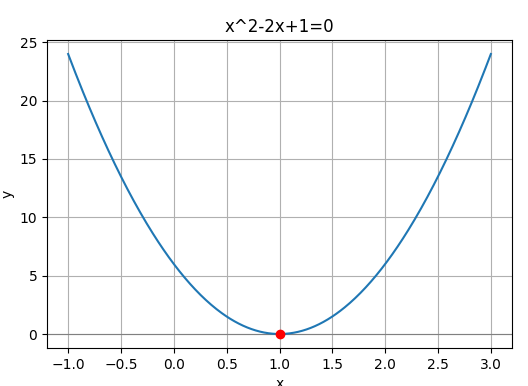
\includegraphics[height=0.4\textheight, keepaspectratio]{figs/parabola.png}
\captionof{figure}{Graph}
\end{figure}
\end{document}